%% ------------------------------------------------------------------------- %%
\chapter{Experimentos de Avaliação de Desempenho do CEP Handler}
\label{cap:experimento}

O desempenho do sistema de processamento de eventos desenvolvido neste trabalho foi avaliado por meio de experimentos executados em uma plataforma de nuvem pública, com uma rede e processamento de eventos para o monitoramento de tráfego de ônibus do sistema de transporte público da cidade de São Paulo, SP. Os detalhes sobre os experimentos são descritos nas seções a seguir.

\section{Caracterização dos Dados de Posição de Ônibus}

Os experimentos usam como entrada dados das posições de ônibus do sistema de transporte público de São Paulo coletados durante três horas contínuas. Os dados foram obtidos por meio da API do sistema \cite{Olhovivo} da São Paulo Transporte S/A (SPTrans), empresa que faz a gestão do sistema de transporte público por ônibus na cidade.
%\todo[inline]{Cabe falar com que frequência os GPSs dos ônibus reportam sua posição, para dar ideia do volume de dados envolvido no problema.}

Os dados foram coletados no dia quatro de novembro de 2019, das 7h57 até às 11h02. Eles se referem a 2.360 linhas de ônibus e 26.624 veículos. O intervalo de tempo médio entre dois envios de dados em cada ônibus é de quinze a vinte segundos.
%, porém escolhemos usar os dados de um terço das linhas de ônibus, de 708 linhas, devido a limitações de processamento pelo rabbitmq.

Os dados coletados foram pré-processados, pois estavam organizados de acordo com as linhas, sendo um dado em JSON para cada linha de ônibus e um campo com um JSON \textit{Array} contendo os dados de cada ônibus servindo a linha. A partir do pré-processamento, os atributos específicos das linhas foram replicados para cada dado de ônibus.
Depois do pré-processamento, os dados ficaram com os campos descritos no Exemplo \ref{exp:dadosSPTrans}.

\begin{evento}[h]
\begin{verbatim}
cl - Código identificador da linha, 
sl - Sentido de operação onde 
   1 significa de Terminal Principal para Terminal Secundário e 
   2 de Terminal Secundário para Terminal Principal,
lt0 - Letreiro de destino da linha,
lt1 - Letreiro de origem da linha,
qv - Quantidade de veículos localizados,
p - Prefixo do veículo,
a - Indica se o veículo é (true) ou não (false) acessível 
para pessoas com deficiência,
ta - Indica o horário universal (UTC) em que a localização foi capturada.
    Essa informação está no padrão ISO 8601,
py - Informação de latitude da localização do veículo,
px - Informação de longitude da localização do veículo,
\end{verbatim}
\caption{Descrição dos dados da SPTrans .}
\label{exp:dadosSPTrans}
\end{evento}

\section{Tipos de Evento Detectados}
\label{sec:exp_event_types}
A rede de processamento de eventos criada para o experimento contém cinco categorias de tipos de evento, que detectam problemas de tráfego de ônibus comuns em grandes cidades, tais como lentidão em corredores e agrupamentos de ônibus.
Cada categoria foi implementada em um dos seguintes níveis de granularidade:
\begin{itemize}
    \item um tipo de evento para cada linha de ônibus;
    \item um tipo de evento para cada corredor de ônibus da cidade;
    \item um tipo de evento para cada ônibus.
\end{itemize}

%No envio dos eventos primários foi adicionado um campo "\textit{timestamp}", para registrar o momento de envio do evento.

\begin{figure}[ht]
\centering
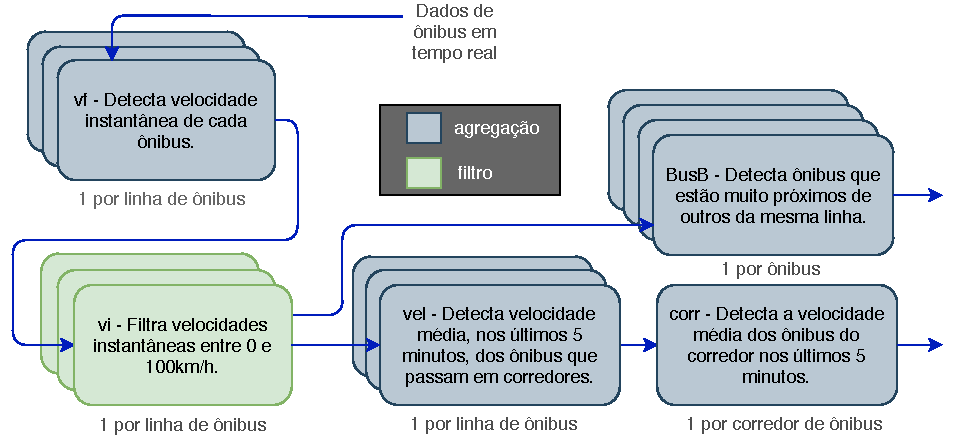
\includegraphics[width=\textwidth]{figuras/diagramadissert.pdf}
\caption{Rede de processamento de eventos de localização de ônibus.}
\label{fig:experiment_diagram}
\end{figure}


A Figura~\autoref{fig:experiment_diagram} mostra o diagrama da rede de processamento, com as origens e destinos de cada categoria de tipo de evento. %\todo[inline]{Fernando, você precisa corrigir a figura. Em vf, a figura dá a entender que a velocidade é calculada por linha (por conta do "agrupado por linha"). Além disso, não tem mais a detecção de velocidades < 20km/h. Veja como ficou as explicações dos tipos de eventos abaixo e tente corrigir a figura de acordo.}
Cada tipo de evento teve seu identificador, que normalmente seria gerado pelo \texttt{CEP Cataloger}, e seu nome criados a partir de prefixos específicos para cada categoria, concatenados ao identificador de linha, ônibus ou corredor. A linguagem EPL do ESPER, utilizada nas definições dos eventos, é bastante similar à linguagem SQL, porém uma diferença significativa é a existência das janelas de agregação deslizantes, como descrito em \autoref{sec:CEPcontext}. Para o experimento foram utilizados dois tipos de janelas:


\begin{itemize}
    \item \textit{ext\_timed}: utiliza um \textit{timestamp} do próprio tipo de evento para realizar a agregação em janelas temporais deslizantes;
    \item \textit{lenght}: utiliza um número de eventos fixo para a agregação por janelas de eventos deslizantes.
\end{itemize}
As definições de janelas de eventos deslizantes e janelas de tempo deslizantes podem ser encontradas em  \autoref{sec:CEPcontext}. 

As cinco categorias de tipos de eventos da rede dos experimentos são: 

\begin{itemize}    
    \item \textbf{Velocidade Instantânea de Ônibus (vf)} -- nível: um por linha de ônibus
    \begin{itemize}
        \item  Id do tipo de evento: vf+(identificador da linha)
        \item Nome do tipo de evento: velf+(identificador da linha)
    \end{itemize}
   
    
    
    Cada tipo de evento nessa categoria calcula a velocidade instantânea de cada ônibus de uma linha, usando a posição recebida e a posição anterior do ônibus. %Portanto, utiliza os últimos dois eventos para cada disparo\todo{a explicação nesta frase não parece correta. O vf não usa os dois últimos eventos que recebeu, mas sim o evento atual + o evento que registrou a posição anterior do ônibus do evento atual, certo? - }.
    
    A definição de \textbf{vf} na linguagem EPL é:
\begin{verbatim}
SELECT cl, p, py, px, ta, timestamp, 
distance(py, px, prev(py), prev(px)) as d,
distance(py, px, prev(py),prev(px))*1000*60*60/Math.abs(ta - prev(ta)) as v,
FROM bus" + cl + "#length(2) group by p 
\end{verbatim}

    Nos experimentos, criou-se um tipo de evento da categoria \textbf{vf} para cada linha de ônibus. Na definição dele, foi utilizado o operador \textit{group by} para separar os eventos por ônibus, já que a função de \textbf{vf} é detectar a velocidade de ônibus (e não de linhas). Na cláusula \texttt{FROM}, pode-se notar que a fonte dos eventos é fixada com o nome de \texttt{``bus''+cl}, sendo \texttt{``cl''} iterado sobre o conjunto de linhas da cidade. 
    
    A função \texttt{distance} utilizada na definição foi adicionada ao código do protótipo, para o cálculo de distancias geodésicas entre coordenadas de latitude e longitude de dois pontos na superfície terrestre em quilômetros. Ela se baseia na fórmula de Haversine para realizar o cálculo~\citep{Haversine}. A velocidade em km/h é calculada pela divisão da distância pela diferença dos \textit{timestamps} \texttt{ta}, convertido para horas.
 
    \item \textbf{Velocidade Instantânea de Ônibus Filtrada (vi)}  -- nível: um por linha de ônibus
    
    \begin{itemize}
        \item Id do tipo de evento: vi+(identificador da linha)
        \item Nome do tipo de evento: veli+(Identificador da linha)
    \end{itemize}
    Cada tipo de evento nessa categoria filtra os eventos de \textbf{vf}, selecionando aqueles que apresentam velocidades entre 0 km/h e 100 km/h. Essa categoria é importante para filtrar possíveis eventos com dados de posição irregulares vindos da SPtrans. 
    
    Em EPL, a definição de \textbf{vi} fica: 
\begin{verbatim}
SELECT cl, p, py, px, d, v, ta, timestamp 
FROM velf" + cl + " 
WHERE v > 0 AND v < 100
\end{verbatim}

%No caso, "velf" é o nome do tipo de evento internamente da ferramenta de CEP.

    \item \textbf{Velocidade Média de Ônibus (vel)} -- nível: um por linha de ônibus que passa em corredores
    
    \begin{itemize}
        \item Id do tipo de evento: vel+(identificador da linha)+(identificador do corredor)
        \item Nome do tipo de evento: speedbus+(Identificador do corredor)
    \end{itemize}
 
    Cada tipo de evento nessa categoria calcula a velocidade média de cada ônibus de uma linha, considerando as velocidades instantâneas do ônibus acumuladas nos últimos 5 minutos. 
    
    Os tipos de evento da categoria \textbf{vel} foram criados somente para as linhas que passam em corredores de ônibus.% , pois servem como eventos de entrada para os tipos de evento da categoria \textbf{corr}.
    
    A definição em EPL dos tipos da categoria \textbf{vel} é:
\begin{verbatim}
SELECT cl,p, py, px,ta,  avg(v) as speed, timestamp 
FROM veli" + cl + "#ext_timed(ta,300) group by p
\end{verbatim}

%"veli" é o nome de \textbf{vi} para a ferramenta de CEP.
%  \item \textbf{corr} - Este evento é disparado quando a velocidade média do corredor de ônibus é menor que 20km/h. A SPTrans considera que corredores com velocidades médias menores que 10km/h já estão apresentando problemas na circulação. Este tipo de evento foi cadastrado um por cada corredor de ônibus na cidade, totalizando 12.
%  Em EPL:
%\begin{verbatim}
%"Select cl, p, py, px,speed , avg(speed) as velocity, ta, timestamp
%FROM speedbus"+corredor+"#ext_timed(ta,300) HAVING avg(speed) < 20"
%end{verbatim}

%\item \textbf{corr} - Este evento é disparado quando um ônibus que das linhas do corredor registra uma velocidade media de menos de 15km/h nos últimos 5 minutos e serve para detectar os pontos geográficos de problemas de trânsito. A SPTrans considera que corredores com velocidades médias menores que 15km/h são indicadores de lentidão na via \cite{DeOlhoNaVia}. Este tipo de evento foi cadastrado um por cada corredor de ônibus na cidade, totalizando 12.

\item \textbf{Velocidade Média em Corredor (corr)} -- nível: um por corredor principal da cidade

\begin{itemize}
    \item Id do tipo de evento: corr+(identificador do corredor)
    \item Nome do tipo de evento: corridor+(Identificador do corredor)
\end{itemize}


Essa categoria de tipos de evento tem como objetivo calcular a velocidade média em cada corredor principal da cidade, a partir das velocidades médias dos ônibus que passam por ele registradas nos últimos 5 minutos. 

No experimento, foram criados 12 tipos de evento dessa categoria, um para cada um dos principais corredores de ônibus de São Paulo.

A definição desses tipos de eventos \textbf{corr} em EPL é:
\begin{verbatim}
SELECT avg(speed) as avg_speed, ta, timestamp 
FROM speedbus"+corredor+"#ext_timed(ta,300)
\end{verbatim}

%No momento do registro da definição de um tipo de evento no sistema de CEP, pode-se escolher  um nome para ele. 
No experimento, para facilitar a definição em EPL dos tipos de evento de \textbf{vel}, registrou-se com um mesmo nome (\texttt{``speedbus''+corredor}) todos os tipos de eventos das linhas que passam num mesmo corredor de ônibus. Desta forma, não foi preciso especificar explicitamente na cláusula \texttt{FROM} a grande lista de tipos de evento de entrada (referentes às várias linhas de ônibus que passam pelo corredor).

\item \textbf{Aglomeração em Linha de Ônibus (BusB)} -- nível: um por ônibus

\begin{itemize}
    \item Id do tipo de evento: BusB+(identificador do ônibus)+(identificador da linha)
    \item Nome do tipo de Evento: BB+(identificador do ônibus)+(identificador da linha)
\end{itemize}

Nessa categoria, um tipo de evento é criado para cada ônibus em circulação, para detectar se existem ônibus da mesma linha circulando muito próximos um do outro. 
Esse é um problema comum em engenharia de transporte público, algo que ocorre com frequência na cidade, e que leva a um tempo desigual de espera entre ônibus da mesma linha. 

A definição em EPL dos tipos de eventos da categoria \textbf{busB} fica: 
  
\begin{verbatim}
"SELECT o.p as op, b.p as bp, o.cl as ocl,b.cl as bcl,o.py as py,
o.px as px, o.v as ov,b.v as bv, o.ta as ota, b.ta as bta,
max(o.timestamp,b.timestamp) as timestamp 
FROM veli" + cl + "(p != " + c + ")#ext_timed(ta,30) as o,
veli" + cl + "(p = " + c + ")#ext_timed(ta,30) as b 
WHERE distance(o.py, o.px, b.py, b.px) < 0.5 AND o.p > b.p"
\end{verbatim}
Os tipos de evento de \textbf{busB} utilizam como entrada os eventos do tipo \textbf{vi}, com duas fontes separadas -- uma só para eventos do ônibus selecionado (\texttt{p = c}) e uma para todos os outros ônibus da mesma linha (\texttt{p != c}) -- e disparam toda vez que dois eventos, um de cada fonte, apresentam uma distância de menos de 500 metros entre si dentro de um intervalo de 30 segundos. A condição \texttt{o.p > b.p} foi adicionada pois, como um tipo de evento de \textbf{busB} é criado para cada ônibus, na ocorrência de um agrupamento de ônibus seriam detectados eventos para ambos os ônibus participantes do agrupamento. Com esta condição, somente o tipo de evento do ônibus com o identificador de maior número é disparado.

\end{itemize}

%\todo[inline]{Nas definições acima, você atribuiu o nome vf ao primeiro tipo de evento. Mas, na definição EPL de vi, usou velf e depois disse que velf é o nome interno de vf. Na definição EPL de corr, usou veli (nome interno) em lugar de vi! Eu tirei velf e veli do texto, pois fica muito confuso usar dois nomes diferentes para uma mesma coisa. Na verdade, o correto aqui seria trocar todos esses nomes por outros mais auto-explicativos e em português. Faça isso se der tempo. - Falotou definir que um é o identificador do tipo de evento e o outro é o nome do tipo de evento}

%\todo[inline]{As definições EPL dos eventos precisam ser melhor explicadas. O texto não explica a sintaxe geral da linguagem. Em particular, seria bom ao menos descrever as funções de criação das janelas (como a ext\_time e length). Em vf, é preciso explicar com o cálculo da velocidade é feito, dizer o que a função distance faz e mencionar a conversão da unidade de tempo. No busB, tem que explicar porque o o.p > b.p e o max(o.timestamp,b.timestamp) estão sendo usados na definição do tipo de evento. }



Para os experimentos, foram usados dados de apenas 708 linhas de ônibus (30\% do total de linhas da cidade), devido a limitações de uso de recursos no cadastro de filas e canais no rabbitmq. Cada experimento utiliza uma só instância do rabbitmq, e para cada tipo de evento registrado é necessária a inscrição da instância no rabbitmq para receber os novos tipos de entrada e enviar os eventos detectados pelo novo tipo cadastrado. As 708 linhas foram escolhidas porque passam pelos corredores de ônibus da cidade e têm a maior quantidade de dados coletados. No total, a rede de processamento para o monitoramento dessas linhas contém 15.729 tipos de eventos, sendo:
\begin{itemize}
    \item 708 tipos para detecção de velocidades instantâneas de ônibus (vf), um por linha;
    \item 708 tipos para filtragem de velocidades entre 0 e 100 km/h (vi), um por linha;
    \item 180 tipos para cálculo de velocidade média de ônibus (vel), um por linha que passa em corredores;
    \item 12 tipos para cálculo de velocidade média em corredor (corr), um para cada corredor principal;
    \item 14.121 tipos para detecção de aglomeração em linha de ônibus (busB), um para cada ônibus.
\end{itemize}

%\todo[inline]{Faltou explicar como as 708 linhas foram escolhidas entre as demais. }

\section{Arquitetura dos Experimentos}
\label{sec:experiment_architecture}
Para simular um ambiente de execução do sistema \texttt{CEP Handler} de forma automatizada, foi projetado um microsserviço adicional, o \texttt{Experiment-Repository} (\cite{Experiment-Repository}), cuja função é o envio dos eventos primários e a coleta e armazenamento de todos os eventos detectados. A arquitetura do ambiente dos experimentos é representada em \autoref{fig:experiment_arch_diagram}.
O banco de dados chave-valor que é consultado pelo \texttt{CEP Worker} para o cadastro e verificação dos metadados dos tipos de eventos é instanciado já com todos os metadados dos tipos de eventos da rede de processamento dos experimentos pré-registrados.

O microsserviço de experimento carrega todos os dados dos eventos primários de um arquivo para a memória RAM antes do início do experimento e depois os ordena pela marca temporal \textit{"ta"} (do horário em que a posição do ônibus foi capturada no sistema da SPTrans), para enviá-los um por vez ao \texttt{CEP Handler}. Um evento primário $E_t$ só é enviado pelo \texttt{Experiment-Repository} ao \texttt{CEP Handler} quando o intervalo de tempo transcorrido desde o envio do evento anterior $E_{t-1}$ for igual ao intervalo entre os tempos $E_t.ta$ e $E_{t-1}.ta$. 
Dessa forma, o microsserviço de experimento simula o envio de eventos na mesma taxa provida pela SPTrans. 
Além disso, no envio dos eventos primários, é adicionado um atributo novo, chamado \textit{"timestamp"}, que contém a marca temporal do envio do evento pelo microsserviço. Quando o microsserviço coleta os eventos detectados, ele armazena a marca temporal de saída do evento do sistema. Com as duas marcas temporais, é possível calcular a latência da detecção dos eventos no sistema \texttt{CEP Handler} posteriormente.  

%\todo[inline]{É preciso dizer nesta seção que dois experimentos diferentes foram realizados, um para cada um dos algoritmos de balanceamento de carga apresentados no cap. 4, e que ambos foram repetidos 5 vezes. -  o número de repetições faz parte da denição teórica de como o experimento deve ocorrer? Acho que o numero de repetições de execução está mais associado a coleta de resultados que a montagem do experimento}


\begin{figure}[tb]
\centering
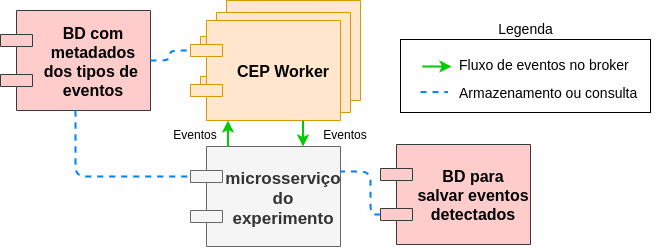
\includegraphics[width=\textwidth]{figuras/arquiteturaexp.png}
\caption{Arquitetura de processamento dos experimentos.}
\label{fig:experiment_arch_diagram}
\end{figure}

\section{Ambiente de Execução} 
A execução dos experimentos foi feita na plataforma de nuvem Amazon Web Services (AWS), com créditos concedidos ao projeto CNPq/AWS Nº 032/2019, intitulado ``Computação em nuvem para big-data em cidades inteligentes''.
%Ela foi escolhida pois o projeto InterSCity recebeu um aporte de créditos para a implantação na nuvem da plataforma de cidades inteligentes utilizando os recursos da AWS. 
A ferramenta eksctl \citep{EKSCTL} foi usada para fazer a interface entre o orquestrador de contêineres Kubernetes, utilizado pelo \texttt{CEP Handler}, e os recursos providos pela AWS.

Cada um dos microsserviços foi alocado em uma máquina virtual do tipo t3a.medium da AWS, com 2 vCPU, 4 GB de memória RAM e até 5 Gbps de desempenho na rede \citep{AWSTypes}. Esse tipo de máquina virtual foi escolhido por representar uma máquina virtual comum, que poderia ser encontrada em qualquer provedor de nuvem.

%\todo[inline]{É preciso dizer que a cada nova execução de um dos experimentos, todo o ambiente era recriado do zero, para garantir que nenhum efeito de cache interferisse no desempenho.}


\section{Execução}
O experimento foi executado dez vezes, cinco para cada um dos algoritmos de balanceamento de carga apresentados no Capítulo \ref{cap:arquitetura}. A cada nova execução, todo os recursos do ambiente de nuvem eram removidos e requisitados novamente.

%Os dados coletados representam 3 horas contínuas de fluxo durante o período da manha, quando a frota de ônibus está aumentando. Para cada um dos algoritmos de realocação, descritos em \autoref{sec:loadDistribution}, o experimento foi repetido cinco vezes.





